%!TEX root = Thesis.tex
\chapter{Background}\label{cha:background}
    In order to be able to solve the given problem we will have to rely on several
    well known approaches, which I will briefly introduce in this chapter.
    \section{Occupancy Grids}\label{sec:occupancy_grids}

        In this thesis we partly
        make use of the grid maps to model the environment with respect to modeling
        the probability of cars to be present in the particular part of the world.
        Grid maps partition the space into a grid of rectangular cells. Each grid
        contains information about the corresponding area in the environment. In this
        thesis we make use of one particular realization of grid maps --- the
        occupancy grid maps. Occupancy grid maps assume that each grid cell is either
        occupied by an obstacle or free. In our case, each cell therefore stores the
        probability that the particular cell is occupied by a car. The occupancy grid
        maps are an efficient approach for representing uncertainty. Grid maps allow
        for detailed representation of an environment without a predefined feature
        extractor. As they have the ability to represent occupied space, empty space
        and unknown (unobserved) space, grid maps are well suited for tasks such as
        path-planning, obstacle avoidance and exploration. In contrast to most
        representations based on features, grid maps offer constant time access to
        cells. However, grid maps suffer from discretization errors.

    \section{Object Detection}\label{sec:object_detection}
        \begin{figure}[th]%
            \centering
            \subfloat{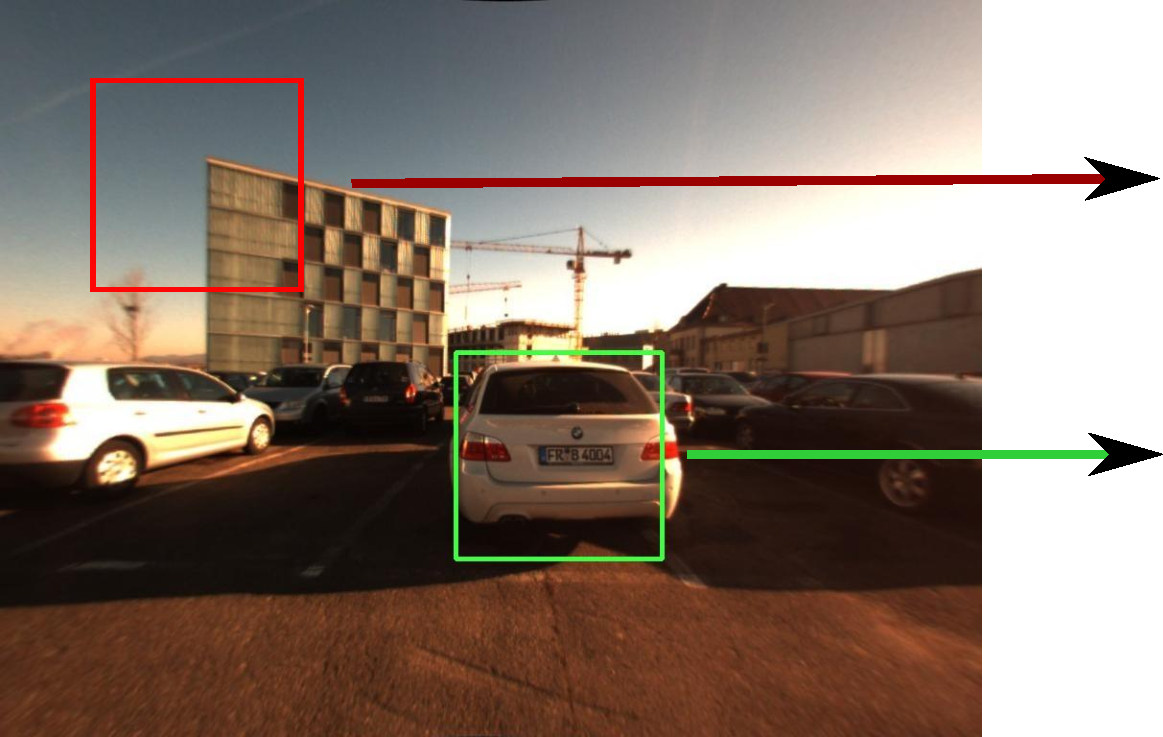
\includegraphics[width=0.35\textwidth]{pictures/detections.pdf}}
            \subfloat{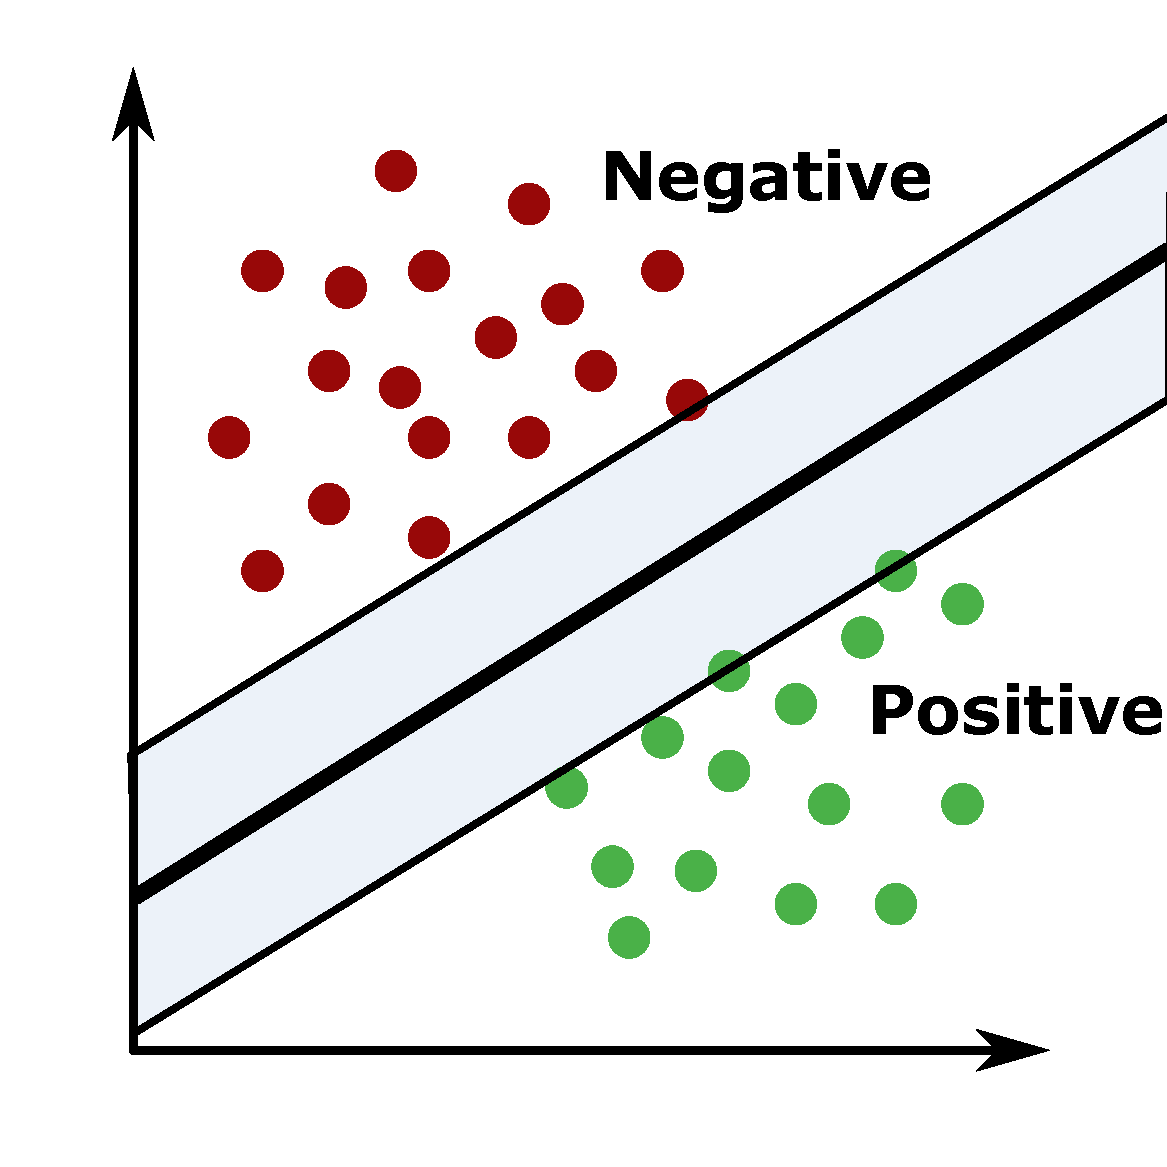
\includegraphics[width=0.35\textwidth]{pictures/svm.pdf}}\\
            \subfloat{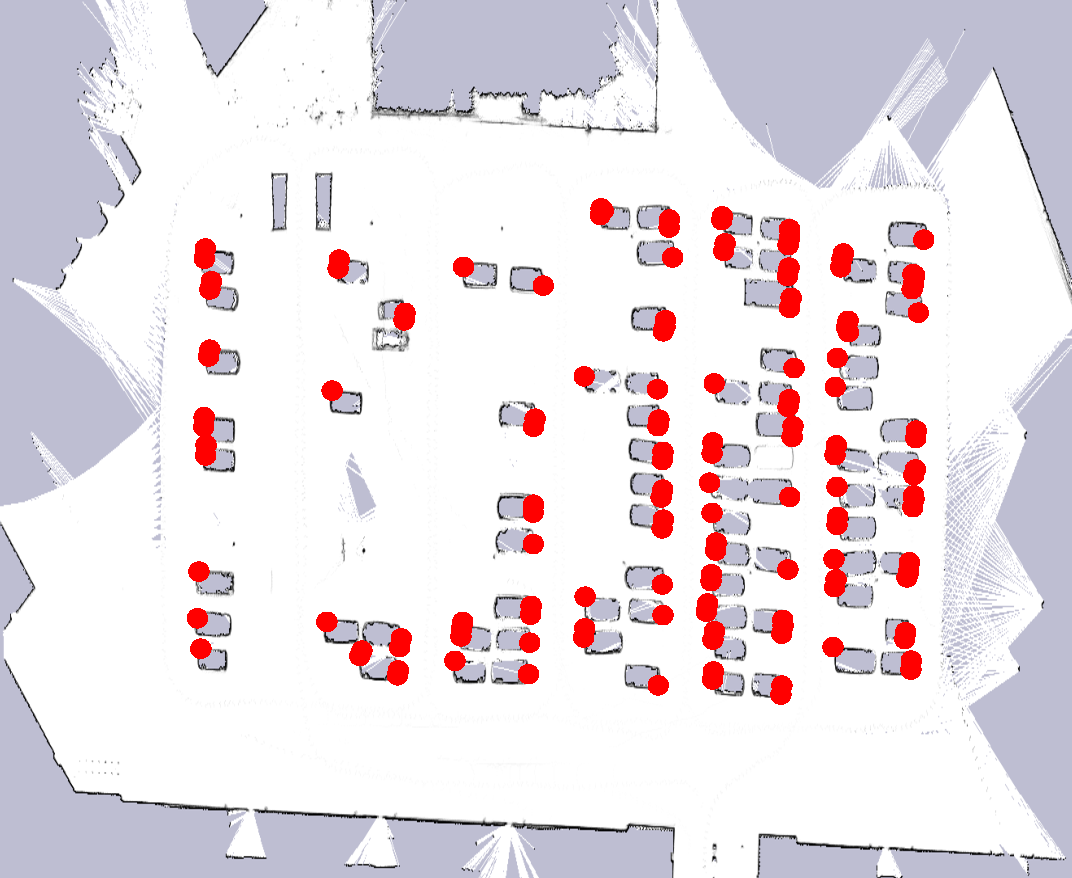
\includegraphics[width=0.4\textwidth]{pictures/laser_fusion.pdf}}
            \caption{Illustration of HOG-based detection and clustering with SVM.}
            \label{fig:det_to_svm}
        \end{figure}
        In this thesis we make extensive use of the object detection to be able to
        detect parked cars from visual information. Based of the work
        of~\cite{dalal2005} we make use of the histograms of oriented gradients
        (HOG) features placed in a dense grid on the query images. The histograms
        from the training data, describing positive and negative sets are then
        divided into positive and negative groups via support vector machines
        (SVM), presented by~\cite{svm2003}, as shown in Figure~\ref{fig:det_to_svm}.

        Let us shortly describe how the HOG descriptor is formed. The image is
        partitioned into $8 \times 8$ pixel blocks. In each block we compute the
        histogram of the gradient orientations. This histogram, after the
        normalization is invariant to changes in light, small deformations etc.

        The HOG/SIFT representation has several advantages. It captures edge or
        gradient structure that is very characteristic of local shape, and it does
        so in a local representation with an easily controllable degree of
        invariance to local geometric and photometric transformations:
        translations or rotations make little difference if they are much smaller
        than the local spatial or orientation bin size.


    \section{Markov Decision Processes}\label{sec:markov_descision_processes}
        Markov decision processes are used to carry out complex decisions in a fully
        observable environment with a stochastic transition model.
        A specification of the outcome probabilities for each action in each possible state is
        called a transition model, we will use $T(s| s', a)$ to denote the
        probability of reaching state $s'$ if and action $a$ is carried out in state
        $s$.
        The transitions in the model are assumed to be Markovian. That is, the probability of
        reaching $s'$ from $s$ depends only on $s$ and not on the history of earlier
        states.
        We also need to define the reward function $R(s, a, s')$, that defines a reward
        for reaching state $s'$ from state $s$ carrying out action $a$.
        Overall, the MDP is defined by three components:
        \begin{itemize}
            \item Initial state: $S_0$
            \item Transition Model: $T(s| s', a)$
            \item Reward Function: $R(s, a, s')$
        \end{itemize}
        These components allow us to define the utility function, which is a measure of
        how good the state is in the long run:
        \begin{equation}
        U^{\pi}(s) = E\left[\sum_{t=0}^{\infty} \gamma^t R(s_t) | \pi,s_0 = s \right]
        \end{equation}
        The optimal action is then chosen using the Maximum Utility Principle, that is,
        choose: the action that maximizes the expected utility of the subsequent state:
        \begin{equation}
        \label{lbl:optimal_policy}
        \pi^*(s) = \argmax_a \sum_{s'} T(s| s', a)U(s')
        \end{equation}
        Provided, that the utility of the state is the expected sum of discounted
        rewards from that point onwards, we can define the utility via Bellman Equation:
        \begin{equation}
        \label{lbl:bellman_equation}
            U(s) = R(s) + \gamma \max_a \sum_{s'}T(s| s', a)U(s')
        \end{equation}
        In order to solve the MDP there are two common strategies to be used:
        \begin{itemize}
            \item Variable iteration
            \item Policy iteration
        \end{itemize}
        In this thesis we will only focus on the second, which is briefly introduced here. \\
        The policy iteration algorithm alternates the following two steps, beginning from some initial policy $\pi_0$,
        \begin{itemize}
            \item \emph{Policy evaluation:} given a policy $\pi_i$, calculate $U_i = U^{\pi_i}$, the utility of each state if $\pi_i$, were to be executed.
            \item \emph{Policy improvement:} Calculate a new MEU policy $\pi_{i+l}$, using one-step look-ahead based on $U_i$ (as in Equation~\ref{lbl:optimal_policy}).
        \end{itemize}
        The algorithm terminates when the policy improvement step yields no change in the utilities. The given method can be shown to converge in $O(n^3)$.
% chapter background (end)



